% ##################################################################################################################
\chapter{The SmartBay Project: Connected Mobility in San Francisco Bay Area}
\label{ch:sanfrancisco}
\hfill \textbf{Author:} Alexei Pozdnoukhov, Andrew Campbell, Sidney Feygin, Mogeng Yin, Sudatta Mohanty

% ##################################################################################################################
\section{Introduction}
Novel mobility-as-a-service paradigm, enabled by \gls{ict} and mobile computing, is changing the transportation landscape quicker than traditional data sources, such as travel surveys, are able to reflect. The development of on-demand transportation, the rising popularity of car- and ride-sharing services and the growing tendencies towards multi-modality pose new challenges on the supply side modeling. This is particularly true in the San Francisco Bay Area (California, USA) as the influx of citizens and businesses to the city, the volatility of job markets, evolving demographics and internal migration further increase the variability of the evolution of mobility patterns. It is more important than ever to be able to measure, realistically model and forecast travel demand in near real-time. The baseline scenario of the SmartBay project spans the nine counties of the area and is designed to extend the state-of-the-art in activity-based simulations in two respects. First, the SmartBay’s demand model is based on the anonymized data stream from the cellular network infrastructure. Second, the agents' population is connected into a social network and their scoring functions are tailored to study the implications social influence effects, particularly in mode and secondary destinations locations choice. 

 %------------
\createfigure%
{The geographical extent of the SmartBay simulation (left) and a close-up view on the \gls{multimodal} network spanning San Francisco-Oakland area (right).}%
{The geographical extent of the SmartBay simulation (left) and a close-up view on the \gls{multimodal} network spanning San Francisco-Oakland area (right).}%
{\label{fig:sf1}}%
{%
 \createsubfigure%
 {}
 {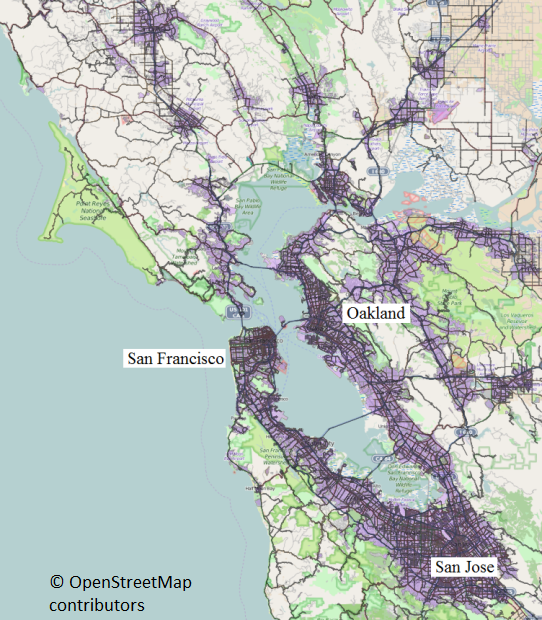
\includegraphics[width=0.44\textwidth, angle=0]{./scenarios/figures/sf_fig1_left.png}}
 {\label{fig:sf_fig1_left}}
\createsubfigure%
 {}
 {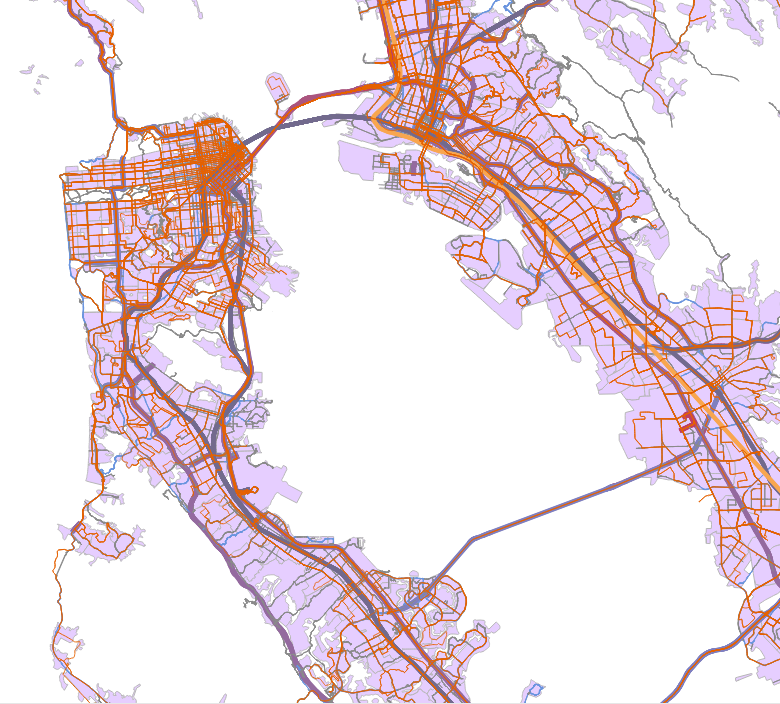
\includegraphics[width=0.54\textwidth, angle=0]{./scenarios/figures/sf_fig1_right.png}}
 {\label{fig:sf_fig1_right}}
}%
{}
 %------------
% ##################################################################################################################
\section{The Study Area and Networks}
The baseline SmartBay simulation implements a scenario of a typical working day within the nine counties of San Francisco Bay Area. As of 2015, the total population of the area is 7.5\,M people, with an estimated 3.4\,M commuters, out of which 350\,K are using public transport as their only commute mode. Driving is the major mode for home to work trips, with 75\,\% of trips made by a driver alone. While the duration of an average commute is estimated to be 28\,minutes, severe congestion at peak hours is widespread. The road network used in the scenario consists of a total of 96\,000\,links, with a mix of freeways, state routes, all major arterial and countryside roads. The road network geometries were extracted from the \gls{osm} data, verified and augmented with the speed limits, capacities and the number of lanes. The network was extended with all major public transit lines available through \gls{gtfs} provided by the respective agencies. There are 9\,major bus agencies, several minor bus line operators, a light rail system, and commuter trains. The major rapid rail carrier is a Bay Area Rapid Transit system that serves 400\,K daily trips over four inter-connected lines. \gls{gtfs} includes the schedules and capacities of transit vehicles.

% ##################################################################################################################
\section{Population and Demand Generation}
There are 1454\,\glspl{taz} in the area developed by the \gls{mtc}, that are used as origin and destination units of a demand model developed and supported by the \gls{mtc}, as well as for population and workplace projections made on a regular basis for different time horizons. The \gls{mtc} model adopts the activity-based approach with a tour-trip hierarchy of mandatory (Home, Work, School trips) and secondary trips, with the respected mode choices, composition of tours and departure times governed by a rich set of discrete choice models calibrated from recent California Household Travel Survey data (CHTS, 2010-2012) and inherited from relevant studies made by other agencies in California. 

SmartBay scenarios use the anonymized cell phone data logs to adjust the \gls{mtc} demand models. The cell phone data are routinely collected and managed by AT\&T Inc., which is the second largest nationwide telecom operator in the United States with 120\,M users nationwide (which translates to a sample size of more than 1\,M commuters in the SF Bay Area). The data used for mobility modeling originates from anonymized \glspl{cdr} recorded at the spatial resolution of the deployed cell phone towers (or antennas) and is usually available with a time latency of several minutes. The analysis of historical \glspl{cdr} allows detection of important places for each user based on the frequency of calls, texts or data packets sent through a given cell tower \citep[][]{IsaacmanEtAl_LNCS_2011, BeckerEtAl_CACM_2013}. This approach is most robust in identifying primary locations of frequent and recurrent visits such as home, work or school. The data is stored and processed internally at secure AT\&T servers. A rescaling procedure based on the area-to-point pycnophylactic interpolation \citep[][]{KaiserEtAl_PMC_2013} and a variant of iterative proportional fitting was used to project the aggregates from the level of cell towers to the areal units defined by the \glspl{taz}. Population census data were used in turn to estimate the correction coefficients and adjust the counts of cell phone users for the total population. This adjustment resulted in an up-to-date and more accurate representation of the \gls{od} flows related to mandatory trips. Notable examples of discrepancies detected as compared with the \gls{mtc} demand models include new urban developments, as well as major shifts in employment re-distribution due to the fast evolution of the IT sector in Silicon Valley.

% ##################################################################################################################
\section{Work Commute Model Evaluation}
\gls{matsim} instance was deployed on AT\&T servers to simulate the home to work commute scenario for a typical weekday. Scenario runs with 15\,\% to 30\,\% sample of the commuting population were evaluated (550\,K to 1.1\,M agents). Driving and public transit were set as the only modes, and the mode share at the beginning of the mode re-planning in \gls{matsim} was set according to the \gls{mtc} findings from CHTS. The resulting link volumes were validated based on the hourly traffic counts collected by inductive loop detectors of the California Department of \gls{pems} deployed at all major freeways. Sample count histograms are presented in Figure~\ref{fig:sf_fig2}. The model was found to meet the Federal Highway Authorities accuracy specifications.

 %------------
\createfigure%
{A sample of the simulated vehicles and the examples of the observed (light/orange) and simulated (dark/blue) counts at two particular validation locations. Secondary trips mainly occurring at midday were not included in this scenario.}%
{A sample of the simulated vehicles and the examples of the observed (light/orange) and simulated (dark/blue) counts at two particular validation locations. Secondary trips mainly occurring at midday were not included in this scenario.}%
{\label{fig:sf_fig2}}%
{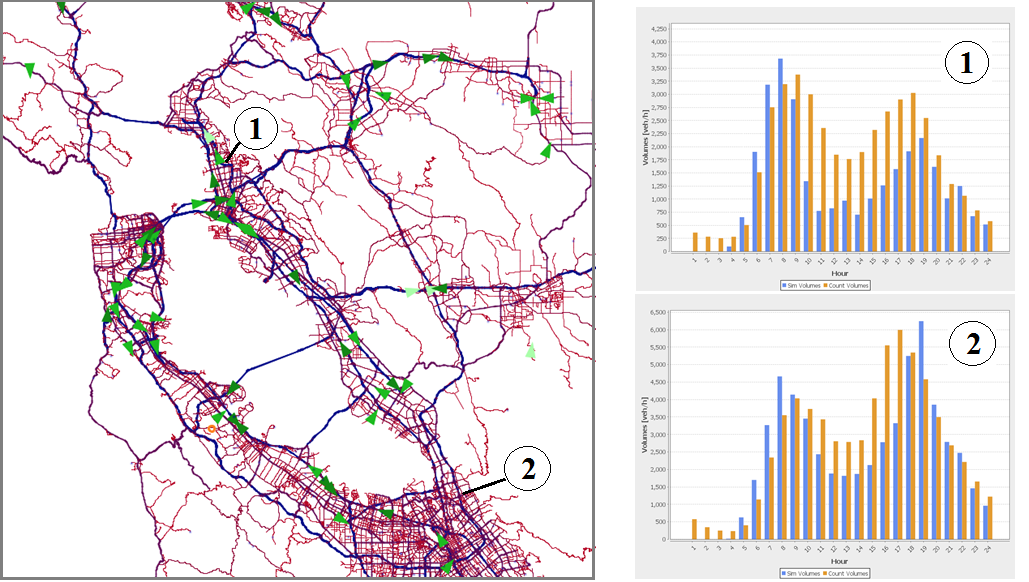
\includegraphics[width=0.99\textwidth, angle=0]{./scenarios/figures/sf_fig2.png}}%
{}
 %------------

% ##################################################################################################################
\section{Extensions and Work in Progress}
The main extensions developed in the SmartBay project are related to simulating a population that is explicitly connected into a social network. There are two domains where the current work is directed towards. First, it is an extension of location choice approached with machine learning tools that model social influences in destination choices for secondary activities. The second extension introduces social connections to scoring functions and aims to capture peer pressure effects in mode choices.

% =============================================================================
\paragraph{Social Influence in Destination Choice}
There is evidence that the geography of the social network of the population in an area is a strong predictor of the destination choice for secondary trips. This is valid both for the trips directly related to social activities, as well as for the cases when destination choice was conditioned by recommendations received from peers in the past. As such, this provides a way to use machine learning-based approaches for predicting destination choice from historical data and social ties. This approach requires building a model of the social connections for the virtual population of agents, \ie defining a weighted graph with edges $P_{ij}$ for each pair of agents $i$ and $j$. Our preliminary work is based on the model proposed in \citet[][]{McGrathPozdnukhov_UrbComp_2014} and is applied at the level of home \glspl{taz} instead of the individuals. This approach requires a seed network to be derived from the cell phone \glspl{cdr}, with the weights $P_{ij}$ emphasizing the recurrent reciprocal calls as an evidence of a social tie between $i$ and $j$. The seed network is then removed from the model, resulting in a connected virtual population having similar network statistics and replicating the geographical community structure of the real social network in the area. 

SmartBay currently adopts the \gls{mtc} classification of the secondary activities that includes eight categories for non-mandatory trips. There are 120\,K venues derived from the \lstinline|Factual.com| \gls{api} and introduced to the simulation as destinations for secondary trips. Hierarchical spatial clustering was applied to the set of venues to reduce the number of venues to 1\,200. This approach is justified both by the need to reduce the computational expenses at re-planning stage, as well as due to an evidence of spatial hierarchies in human spatial cognition and decision making. A spatial choice model for the secondary home- and work-based trips is calibrated from the \glspl{cdr} following the approach of \citet[][]{McArdleEtAl_ACMTIS_2014}. A key set of parameters in this model is the attractiveness of the venues for an agent, which is assumed to be proportional to the number of peers who also visit the venue at hand. A thorough experimental validation of the full-scale scenario with secondary trips is computationally expensive and is ongoing.

% =============================================================================
\paragraph{Social Influence in Mode Choice} 
The following extension to the conventional Charypar-Nagel scoring function is considered:
\begin{equation*}
U_i=U_i^{CN}-\gamma\sum_{j=1}^N P_{ij}\left\Vert a_i - a_i^0 \right\Vert +\theta \sum_{j=1}^N P_{ij} \left\Vert a_i - a_j \right\Vert
\end{equation*}

Here, an agent specification is extended with an attribute vector $a_i$ that describes agent's profile in relation to the membership in a particular group (such as drivers or transit users). We define attribute components to be continuous within $\left[0, 1\right]$ interval, corresponding to an agent's tendency towards driving or transit as his/her primary commute mode. This attribute value is also used to define the probability of the current plan's primary mode choice to be selected for mutation in the evolutionary optimization re-planning step. $U_i^{CN}$ represents the Charypar-Nagel score of the daily plan, which is augmented with two terms. The first term describes peer pressure effect towards a pre-specified ``socially-responsible'' choice $a_i^o$. The second term describes a tendency of an agent to behave similarly to his/her immediate peers with respect to the choice attributes. As both effects are only at work when there is an evidence of a social tie, both terms include a summation over the agent peers, with connection strength $P_{ij}$ defined as described in the previous subsection. The sensitivity of the resulting mode choice to parameters values $\gamma$ and $\theta$ is determined through computational experimentation that is a subject of the ongoing work.

% ##################################################################################################################
\section{Conclusions and Acknowledgments}
An increasing pace of urbanization puts city infrastructure systems under severe test. The field of transportation is responding to these global challenges by evolving at an ever-increasing pace. More flexible and powerful tools are required to support decision making in planning, operations, and policy regulation applied to emerging mobility technologies. SmartBay project develops a \gls{matsim}-based platform that is capable of ingesting demand models based on big data. It extends the utility functions specifications to study social influence in mobility behaviors. It also incorporates semi-parametric machine learning models applied to destination location choice predictions for socially-related secondary trips. With encouraging results obtained in baseline scenario simulations, these advanced developments are currently ongoing. 

The authors acknowledge the contributions from our collaborators at AT\&T Research: Dr.~J.-F.~Paiement, Dr.~J.~Pang, Dr.~A.~Skudlark, Dr.~C.~Volinsky. Funding support from State of California Department of Transportation (CalTrans) through UCCONNECT faculty research grant program, agreement 65A0529, is also acknowledged.

% ##################################################################################################################     




